\documentclass{article}

\usepackage{booktabs}
\usepackage[bottom=3cm]{geometry}
\usepackage{changepage}
\usepackage{tikz}
\usetikzlibrary{er, positioning}

\title{ER schema}
\author{Pietro Jomini}
\date{Maggio 2021}

\begin{document}

\pagenumbering{gobble}
\maketitle
\vspace{1cm}
\tableofcontents
\newpage
\pagenumbering{arabic}

\section{ER schema}

\begin{adjustwidth}{-1cm}{-1cm}
    \vspace{\fill}
    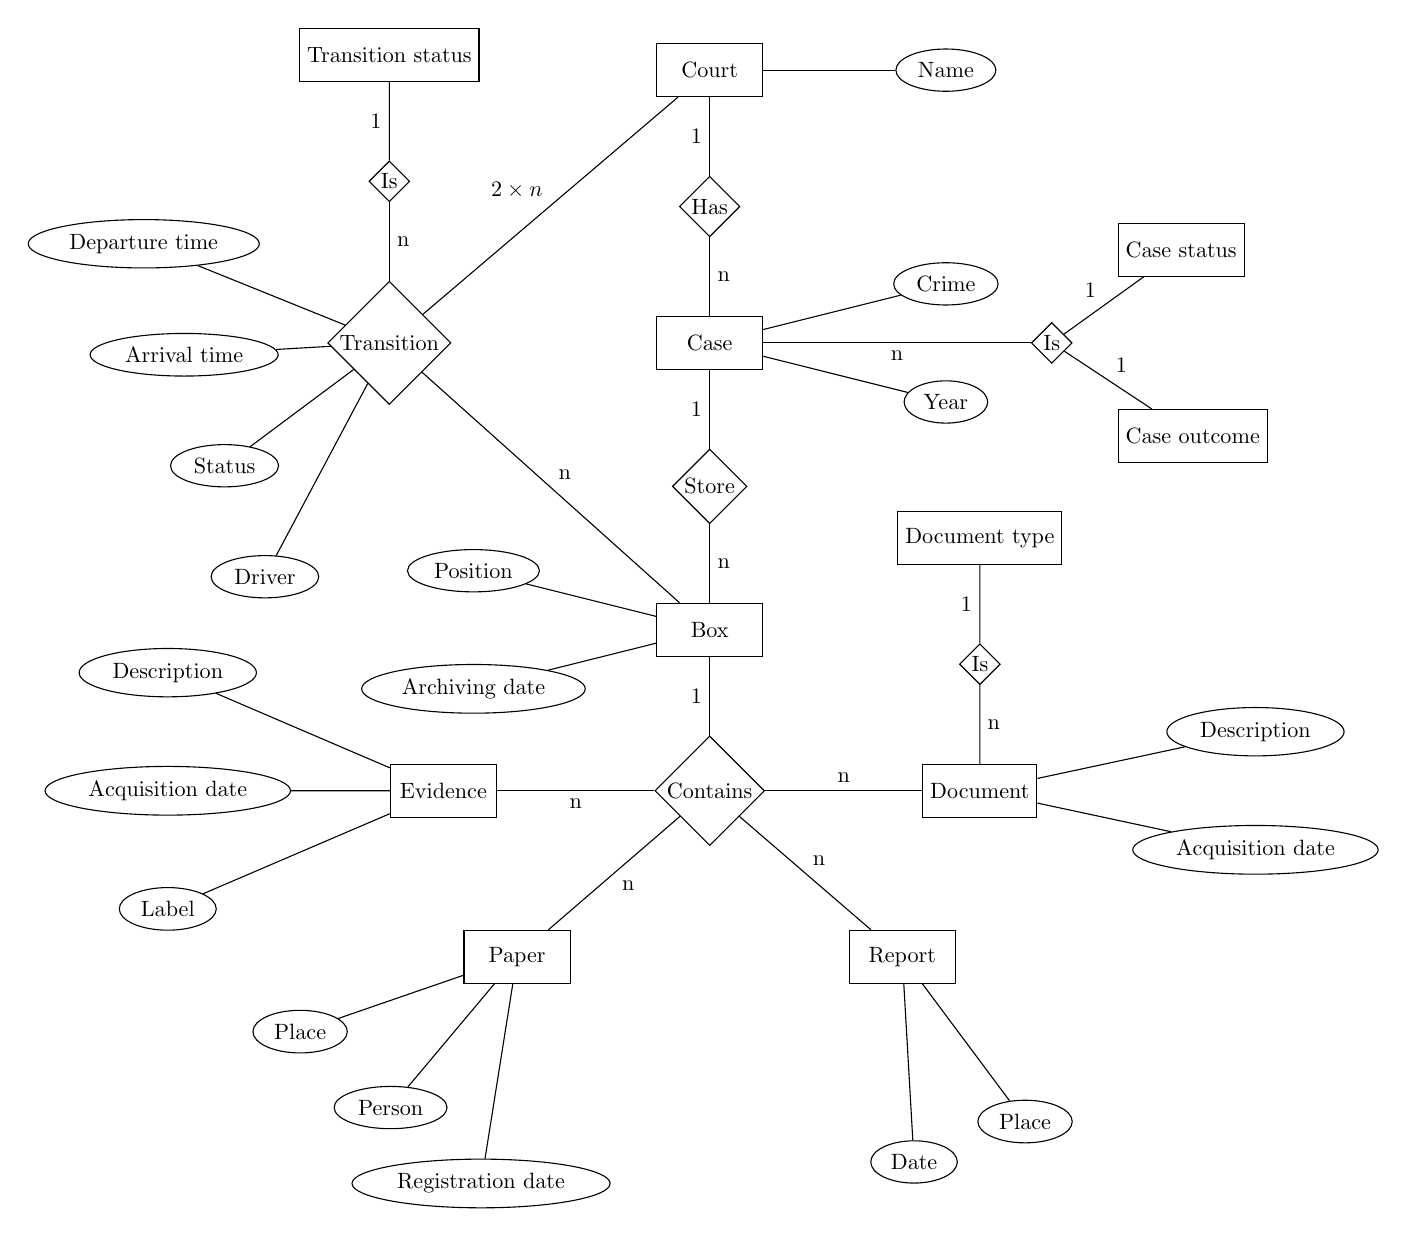
\begin{tikzpicture}[auto, node distance=1cm,scale=1, every node/.style={scale=0.8}]

        % court
        \node[entity] (court) {Court}
        [grow=right, level distance=3cm]
        child {node[attribute] {Name}};

        % case
        \node[relationship] (court_case) [below = of court] {Has};
        \node[entity] (case) [below = of court_case] {Case}
        [grow=right, level distance=3cm]
        child {node[attribute] {Year}}
        child {node[attribute] {Crime}};

        % case status
        \node[relationship] (case_is) [right = of case, xshift=3cm] {Is};
        \node[entity] (case_status) [above right = of case_is] {Case status};
        \node[entity] (case_outcome) [below right = of case_is] {Case outcome};
        \path(case_is) edge node {1} (case_status);
        \path(case_is) edge node {1} (case_outcome);
        \path(case_is) edge node {n} (case);

        % box
        \node[relationship] (case_box) [below = of case] {Store};
        \node[entity] (box) [below = of case_box] {Box}
        [grow=left, level distance=3cm]
        child {node[attribute] {Position}}
        child {node[attribute] {Archiving date}};

        % items
        \node[relationship] (box_item) [below = of box] {Contains};
        \begin{scope}[node distance=2cm]

            \node[entity] (item_1) [left = of box_item] {Evidence}
            [grow=180, level distance=3.5cm]
            child {node[attribute] {Description}}
            child {node[attribute] {Acquisition date}}
            child {node[attribute] {Label}};

            \node[entity] (item_2) [below left = of box_item] {Paper}
            [grow=230, level distance=2.5cm]
            child {node[attribute] {Place}}
            child {node[attribute] {Person}}
            child {node[attribute] {Registration date}};

            \node[entity] (item_3) [below right = of box_item] {Report}
            [grow=290, level distance=2.5cm]
            child {node[attribute] {Date}}
            child {node[attribute] {Place}};

            \node[entity] (item_4) [right = of box_item] {Document}
            [grow=0, level distance=3.5cm]
            child {node[attribute] {Acquisition date}}
            child {node[attribute] {Description}};

        \end{scope}

        % document type
        \node[relationship] (document_is) [above = of item_4] {Is};
        \node[entity] (document_type) [above = of document_is] {Document type};

        % paths
        \path(court_case) edge node {1} (court) edge node {n} (case);
        \path(case_box) edge node {1} (case) edge node {n} (box);

        % items paths 
        \path(box_item) edge node {1} (box);
        \path(box_item) edge node {n} (item_1);
        \path(box_item) edge node {n} (item_2);
        \path(box_item) edge node {n} (item_3);
        \path(box_item) edge node {n} (item_4);

        % document type paths
        \path(document_is) edge node {n} (item_4);
        \path(document_is) edge node {1} (document_type);

        % transition
        \node[relationship] (transition) [left = of case, xshift=-2cm] {Transition}
        [grow=200, level distance=2.5cm]
        child {node[attribute] {Departure time}}
        child {node[attribute] {Arrival time}}
        child {node[attribute] {Status}}
        child {node[attribute] {Driver}};

        % transition paths
        \path(transition) edge node {$2 \times n$} (court);
        \path(transition) edge node {n} (box);

        % transition status
        \node[relationship] (transition_is) [above= of transition] {Is};
        \node[entity] (transition_status) [above = of transition_is] {Transition status};
        \path(transition_is) edge node {1} (transition_status);
        \path(transition_is) edge node {n} (transition);

    \end{tikzpicture}
    \vspace{\fill}
\end{adjustwidth}

\newpage
\section{Enumerable values}

\subsection{Transition status}
\begin{table}[h]
    \begin{center}
        \begin{tabular}{c|l}
            \toprule
            \textbf{Value} &
            \textbf{Description}                                           \\
            \midrule
            Requested      & The destintion court requested the transition \\
            Accepted       & The origin court accepted the transition      \\
            Transiting     & The transition is taking place                \\
            Completed      & The transition is completed                   \\
            \bottomrule
        \end{tabular}
    \end{center}
\end{table}

\subsection{Case status}
\begin{table}[h]
    \begin{center}
        \begin{tabular}{c|c}
            \toprule
            \textbf{Value} &
            \textbf{Description} \\
            \midrule
            Preliminary    & -   \\
            First          & -   \\
            Second         & -   \\
            Canceled       & -   \\
            Prescribed     & -   \\
            \bottomrule
        \end{tabular}
    \end{center}
\end{table}

\subsection{Case outcome}
\begin{table}[h]
    \begin{center}
        \begin{tabular}{c|c}
            \toprule
            \textbf{Value} &
            \textbf{Description} \\
            \midrule
            Condemned      & -   \\
            Acquitted      & -   \\
            \bottomrule
        \end{tabular}
    \end{center}
\end{table}

\end{document}
